\documentclass[final]{article}


% if you need to pass options to natbib, use, e.g.:
%     \PassOptionsToPackage{numbers, compress}{natbib}
% before loading neurips_2024


% ready for submission
\usepackage[nonatbib]{neurips_2024}


% to compile a preprint version, e.g., for submission to arXiv, add add the
% [preprint] option:
%     \usepackage[preprint]{neurips_2024}


% to compile a camera-ready version, add the [final] option, e.g.:
%     \usepackage[final]{neurips_2024}


% to avoid loading the natbib package, add option nonatbib:
%    \usepackage[nonatbib]{neurips_2024}


\usepackage[utf8]{inputenc} % allow utf-8 input
\usepackage[T1]{fontenc}    % use 8-bit T1 fonts
\usepackage{hyperref}       % hyperlinks
\usepackage{url}            % simple URL typesetting
\usepackage{booktabs}       % professional-quality tables
\usepackage{amsfonts}       % blackboard math symbols
\usepackage{nicefrac}       % compact symbols for 1/2, etc.
\usepackage{microtype}      % microtypography
\usepackage{xcolor}         % colors

% Own packages
\usepackage{listings}
\usepackage{amsmath}
\usepackage{graphicx}
\usepackage[
    backend=biber,
    %style=authoryear-icomp,
    %sortlocale=de_DE,
    natbib=true,
    %url=false, 
    %doi=true,
    %eprint=false
]{biblatex}
\addbibresource{transformers.bib}


\title{Formatting Instructions For NeurIPS 2024}
\title{Introduction to Sequence Modeling with Transformers}


% The \author macro works with any number of authors. There are two commands
% used to separate the names and addresses of multiple authors: \And and \AND.
%
% Using \And between authors leaves it to LaTeX to determine where to break the
% lines. Using \AND forces a line break at that point. So, if LaTeX puts 3 of 4
% authors names on the first line, and the last on the second line, try using
% \AND instead of \And before the third author name.


\author{%
  Joni-Kristian K{\"a}m{\"a}r{\"a}inen\thanks{See \url{https://webpages.tuni.fi/vision/public_pages/JoniKamarainen/}}\\
  Department of Computing Sciences\\
  Tampere University
  %\texttt{hippo@cs.cranberry-lemon.edu} \\
  % examples of more authors
  % \And
  % Coauthor \\
  % Affiliation \\
  % Address \\
  % \texttt{email} \\
  % \AND
  % Coauthor \\
  % Affiliation \\
  % Address \\
  % \texttt{email} \\
  % \And
  % Coauthor \\
  % Affiliation \\
  % Address \\
  % \texttt{email} \\
  % \And
  % Coauthor \\
  % Affiliation \\
  % Address \\
  % \texttt{email} \\
}

%\author{%
%  David S.~Hippocampus\thanks{Use footnote for providing further information
%    about author (webpage, alternative address)---\emph{not} for acknowledging
%    funding agencies.} \\
%  Department of Computer Science\\
%  Cranberry-Lemon University\\
%  Pittsburgh, PA 15213 \\
%  \texttt{hippo@cs.cranberry-lemon.edu} \\
%  % examples of more authors
%  % \And
%  % Coauthor \\
%  % Affiliation \\
%  % Address \\
%  % \texttt{email} \\
%  % \AND
%  % Coauthor \\
%  % Affiliation \\
%  % Address \\
%  % \texttt{email} \\
%  % \And
%  % Coauthor \\
%  % Affiliation \\
%  % Address \\
%  % \texttt{email} \\
%  % \And
%  % Coauthor \\
%  % Affiliation \\
%  % Address \\
%  % \texttt{email} \\
%}


%% MY DEFINITIONS
%\lstdefinestyle{mystyle}{
%  belowcaptionskip=1\baselineskip,
%  breaklines=true,
%  frame=single,
%  xleftmargin=\parindent,
%  language=Python,
%  showstringspaces=false,
%  basicstyle=\ttfamily,
%  keywordstyle=\bfseries\color{green!40!black},
%  commentstyle=\itshape\color{purple!40!black},
%  identifierstyle=\color{blue},
%  stringstyle=\color{orange},
%  moredelim=**[is][\color{red}]{@}{@},
%}
%
%\lstset{language=Python,style=mystyle} 
\lstset{language=Python, basicstyle=\scriptsize} 


\begin{document}


\maketitle


\begin{abstract}
  Understanding the transformer architecture and its workings is
  essential for machine learning (ML) engineers. However, truly
  understanding the transformer architecture can be demanding, even if
  you have a solid background in machine learning or deep
  learning. The main working horse is attention, which yields to the
  transformer encoder-decoder structure. However, putting attention
  aside leaves several programming components that are easy to
  implement but whose role for the whole is unclear. These components
  are 'tokenization', 'embedding' ('un-embedding'), 'masking', and
  'positional encoding'. The focus of this work is on understanding
  them. To keep things simple, the understanding is built
  incrementally by adding components one by one, and after each step
  investigating what is doable and what is undoable with the current
  model. Simple sequences of zeros (0) and ones (1) are used to study
  the workings of each step.
\end{abstract}

\begin{center}
\texttt{Jupyter notebook available at} \url{https://github.com/kamarain/transformer_intro}
\end{center}

\section{Background}
If you already know \textit{machine learning} and
\textit{sequence modeling} well, then this section can be skipped. The
purpose of this section is to 
cover the terminology and concepts used in the work.

\paragraph{Supervised machine learning.}
The supervised machine learning problem is to find a model $f$ that
maps inputs $x$ to outputs $y$
\begin{equation}
  y = f(x) \enspace .
  \label{eq:supervisedML}
\end{equation}
The conventional methods for the ML problem are regression and classification.
Before the recent deep learning methods,
the most popular neural ML model was Multilayer Perceptron (MLP). The
fundamental ideas and methods of conventional ML including MLPs are
well covered in Bishop's ML book from 2006~\cite{MLBook}
(available online).

Using the deep learning terminology, MLP is a neural network of
\textit{fully connected layers} and \textit{non-linear activation
  functions} (such as ReLU or Sigmoid) between them. Through the
layers, MLP maps inputs $x$ to outputs $y$. Each neuron (\textit{unit}
or \textit{kernel}) has weights which are the learnable
parameters $\theta$ of the network. Network training is based on
adjusting the weights so that some error (\textit{loss function})
is minimized. The typical loss function for regression is the Mean
Squared Error (MSE) and for classification Cross Entropy (CE). The MSE
loss is defined
\[
\mathcal{L}_{MSE} = \sum_{i=1}^{K} (y_i-f_\theta (x))^2 \enspace .
\]


The loss is computed for a set of $K$ input-output pairs, which is
the \textit{training data}. Formally, the optimization is defined
as
\[
\theta = \arg\min_{\theta} \mathcal{L}_{MSE} \enspace ,
\]
and the standard technique for optimization is the Stochastic Gradient
Descent (SGD) algorithm. The process of passing the loss gradient
through the network is called \textit{error backpropagation}.

A Torch-style code block of a two-layer MLP network:
\begin{lstlisting}
.init(self, input_dim, hidden_size, output_dim):
        self.dense1 = torch.nn.Linear(input_dim, hidden_size)
        self.dense2 = torch.nn.Linear(hidden_size, hidden_size)
        self.output = torch.nn.Linear(hidden_size, output_dim)

.forward(self, x):
    x = self.dense1(x)
    x = torch.nn.functional.sigmoid(x)
    x = self.dense2(x)
    x = torch.nn.functional.sigmoid(x)
    y_pred = self.output(x)
    return y_pred
\end{lstlisting}



\paragraph{Sequence modeling.}
A problem domain where sequence modeling is used is time series
forecasting. For example, forecasting future stock prices is a time
series forecasting application. The problem can be defined as the
problem of predicting the future values
$\hat{x}_N, \hat{x}_{N+1}, \ldots, \hat{x}_{N+M}$ of a process
from which past values $x_0, x_{1}, \ldots, x_{N-1}$ are known.
The hat symbol $\hat{\cdot}$ is used to distinguish between the true
(ground truth) and predicted values.

An ML-compliant definition is to find the model $f_\theta$ so that
\[
\mathbf{Y} = f_\theta (\mathbf{X}) 
\]
and MLP can be used to find a model. The problem with the MLP model is
that the length of the sequences $\mathbf{X}$ and $\mathbf{Y}$ can vary,
but MLP must have a fixed number of inputs and outputs. For iterative
forecasting, the number of outputs can be set to one, and the number
of inputs can be 'big enough', and if the input sequence is
shorter than the maximum limit, \textit{padding inputs} are added.
However, such a network grows rapidly for an increasing number of
inputs and soon becomes useless for practical applications where only
a limited number of training samples are available.

The number of inputs can be reduced, only one past example being the
limit. In this case, the MLP learns the mapping
\[
x_{n+1} = f_\theta (x_{n}) \enspace ,
\]
but this naïve approach does not work very well. For example, it
cannot model sinusoidal signals since each value except 0 and 1
appears in two ’contexts'; the raisin and falling edges of the wave.
t the same time, it is well known that some problems need to address
both short and long-horizon dependencies to predict the next value.
This problem can be solved by Recurrent Neural Networks (RNNs), in
theory, and by Transformers, in practice.


\paragraph{Sequence-to-sequence (Seq2Seq) modeling.}
In the deep learning literature, Seq2Seq models are discussed with
Recurrent Neural Networks (RNNs). The main difference between the MLP
and RNN models is that RNNs maintain a system 'state' $h_t$ that is
always passed forward to the next prediction. The RNN model can be
defined as
\[
x_{n+1},h_{n+1} = f_\theta (x_{n},h_{n+1}) \enspace .
\]

Theoretically, RNNs can have infinitely long 'memory', but in practice,
that would mean that gradient information would be maintained over a
long period of time, which is difficult with limited precision of
computer arithmetics and time. 

Many RNN architectures have been proposed, and one of the most popular
is Long Short-Term Memory (LSTM)~\cite{LSTM}.


\paragraph{Transformer architecture.}
To understand the design choices of the Transformer architecture, it
can be beneficial to learn about the progression of RNNs in machine
translation where one language is mapped to another
(English-to-French). This Seq2Seq problem is more general than the
time series forecasting since the type of input and output are
different (English vs. French vocabulary).


A very good work that describes the principled idea of using RNNs
(LSTM) in machine translation is~\cite{Sutskever-2014-neurips}.
The encoder LSTM encodes the input sequence of $N$ inputs into the state
variable. In practice, that is the last state $h_n$ of the LSTM. Then
the state vector is passed to the decoder LSTM that starts to generate
output. The starts and ends of both sequences are encoded using
special symbols Start-of-Sequence (SOS) and End-of-Sequence (EOS).

A similar structure was used in~\cite{Cho-2014-emnlp}, which is a good
read after~\cite{Sutskever-2014-neurips}. They note that such a
structure quickly 'forgets' history and propose a mechanism that uses
information from all past samples to infer the next prediction(s).
This mechanism is \textit{attention}. In their model,  all past state
vectors are stored, multiplied by \textit{attention weights}, and
summed for the decoder. Similarly, the decoder can use its previous
outputs via \textit{self-attention}. This approach can use all input samples in
inference, but its main bottleneck is the sequential process of RNNs
which makes training and inference slow. This attention mechanism is
often referred to as \textit{Bahdanau attention}.

Finally, after the two previous and influential works, the seminal
Transformer paper ``Attention is All You Need'' is much easier to
comprehend with all its flavors~\cite{transformer}. The most important
idea is to avoid the sequential processing of RNNs. This is achieved
by multiplicative attention that exploits the neural computation
library (Torch, Keras) functions ability to automatically forward any
number of inputs and backward the gradients from the loss function. In
many ways, Transformer is more like clever software engineering than
new AI theory.


\section{Methods}

In the following sections, we incrementally add the essential
components to the plain transformer and demonstrate how its
capabilities gradually improve in Seq2Seq modeling.

\subsection{Plain Transformer}
\label{sec:PlainTransformer}

At first, we investigate a model with a Transformer as its only
processing layer.
This model is referred to as \texttt{PlainTransformer}.
The experimented transformer follows the original structure
in~\cite{transformer}, and \texttt{torch.nn.Transformer} is selected
as the reference implementation. The public implementation is tested
by many users in the PyTorch community and hides all the
implementation details making it straightforward to use.

The only difference to the original work is feature normalization
which is done \textit{before} the multiheaded attention.
This is done by setting the initialization parameter
\texttt{norm\_first = True}. This setting stabilizes training and no
’heatup’ epochs with increasing learning rates are needed at the
beginning of training.
The change was proposed
in~\cite{Xiong-2020-icml}, and we verified improved training
convergence also in our experiments.

A Torch compliant definition of \texttt{PlainTransformer} is
\begin{lstlisting}
class PlainTransformer(nn.Module):
    def __init__(
        self,
        d_model,
        nhead,
        num_encoder_layers,
        num_decoder_layers,
        dim_feedforward,
        dropout_p,
        layer_norm_eps
    ):
        super().__init__()

        # Transformer initialized with user specs
        self.transformer = nn.Transformer(
            d_model = d_model,
            nhead = nhead,
            num_encoder_layers = num_encoder_layers,
            num_decoder_layers = num_decoder_layers,
            dim_feedforward = dim_feedforward,
            dropout = dropout_p,
            layer_norm_eps = layer_norm_eps,
            norm_first = True
        )

    def forward(
        self,
        src,
        tgt,
    ):
        # Transformer assumes that src & tgt structure is (seq_length, batch_num, feat_dim)
        out = self.transformer(src, tgt)

        return out
\end{lstlisting}

An instance of the \texttt{PlainTransformer} model is constructed
using minimal parameters
\begin{lstlisting}
model = SimplestTransformer(d_model = 1, nhead = 1, num_encoder_layers = 1,
                            num_decoder_layers = 1, dim_feedforward = 8,
                            dropout_p = 0.1, layer_norm_eps = 1e-05)
\end{lstlisting}
For the sake of some learning capacity, 8 units are used in the
Transformer's feedforward layers. With a single unit the number of
learnable parameters is 46, and with 8 units 88 parameters. The
remaining 46 parameters are related to the normalization layers and
other learnable operations.

\paragraph{Training sequences 1.} For simplicity, we train the
transformer with data where the input is repeated in the output:
\begin{displaymath}
  \begin{split}
    \mathbf{X}: 0,0,0,0 \rightarrow \mathbf{Y}: 0,0,0,0\\
    \mathbf{X}: 1,1,1,1 \rightarrow \mathbf{Y}: 1,1,1,1
  \end{split}
\end{displaymath}
Despite that there are only two sample sequences, 50 of each and the total of
100 samples were generated for training.

\paragraph{Results.} PlainTransformer was trained for 300 epochs using
the Adam optimizer with the learning rate set to $0.01$. The final
loss was $0.5$. The converged model was experimented using the
training inputs and outputs, and it produced the following output:
\begin{displaymath}
  \begin{split}
    \mathbf{X}: 0,0,0,0 \rightarrow \hat{\mathbf{Y}}: 0.5,0.5,0.5,0.5\\
    \mathbf{X}: 1,1,1,1 \rightarrow \hat{\mathbf{Y}}: 0.5,0.5,0.5,0.5\\
  \end{split}
\end{displaymath}

\paragraph{Findings.} The transformer encoder is designed to
``cross-correlate'' each input sequence sample with all other
samples. This way the encoder outputs of each sample become aware of
their context. Before the cross-correlated samples are transferred to
the decoder, they go through linear mapping. The purpose of the
mapping is to adjust input features to the output features (note that
they could be of different types). The decoder performs similar
cross-correlation between all inputs and produced outputs. This way
each output feature becomes aware of all inputs and past and future
outputs. Again, a linear mapping layer converts feature
vectors to the space suitable for the loss function.

In our case, the decoder outputs were directly used as the
predictions. There are no non-linear mappings in the processing
pipeline, and therefore the plain transformer converges to
produce a single output that minimizes the error over training data. In
the case of the equal amount of ones and zeros, the best single
estimate is the mean (0.5).

\subsection{Token embedding and un-embedding}

From the results with \texttt{PlainTransformer} in
Section~\ref{sec:PlainTransformer} it is clear that Transformer inputs
and outputs should be used as \textit{embeddings} so that Transformer
can alter them to produce compact feature descriptor of the input and
output sequences.

The Torch class \texttt{torch.Embedding()} can be used to form a
lookup table with learnable parameters (the embedding vectors):
\begin{lstlisting}
class TokenTransformer(nn.Module):
...

        .__init__(...)
        ...
        # Token embedding layer - this takes care of converting integer ids to vectors
        self.embedding = nn.Embedding(num_tokens, d_model)

        # Token "unembedding" to one-hot encoded token vector
        self.unembedding = nn.Linear(d_model, num_tokens)
        ...
        
       .forward(...)
       ...
        # Note: src & tgt default size is (seq_length, batch_num, feat_dim)

        # Token embedding
        src = self.embedding(src) * math.sqrt(self.d_model)
        tgt = self.embedding(tgt) * math.sqrt(self.d_model)        

        # Transformer output
        out = self.transformer(src, tgt)
        out = self.unembedding(out)
        
        return out
\end{lstlisting}
The embedding vectors are multipled by the square root of feature
dimension $\sqrt{D}$ to magnify them depending on the number of
dimensions. The learnable parameters of the embedding increase the
total number of learnable parameters from 88 to 1332 using the
defaults of Torch implementations.

\paragraph{Tokenization.} We need to decide 'tokens' used to represent
our sequence. Tokens are integer values and the natural tokens are
\begin{itemize}
\item 0 for '0' and
\item 1 for '1' .
\end{itemize}
In addition, we now add the Start-of-Sequence (SOS) and
End-of-Sequence (EOS) tokens 
\begin{itemize}
\item 2 for SOS and
\item 3 for EOS .
\end{itemize}
The total number of tokens to be embedded is 4, and the embedding
vector dimension is the same as the Transformer internal model
dimension.

\paragraph{Training sequences 2.} Instead of the two previous
sequences, two new sequence types are experimented,
\begin{displaymath}
  \begin{split}
    \mathbf{X}: 0,0,0 \rightarrow \mathbf{Y}: 1\\
    \mathbf{X}: 1,1,1 \rightarrow \mathbf{Y}: 0
  \end{split}
\end{displaymath}
and
\begin{displaymath}
  \begin{split}
    \mathbf{X}: 1 \rightarrow \mathbf{Y}: 0, 0, 0\\
    \mathbf{X}: 0 \rightarrow \mathbf{Y}: 1, 1, 1
  \end{split} \enspace
\end{displaymath}
i.e. three-to-one and one-to-three. Again, 100 samples are generated.

\paragraph{Results.}
\texttt{TokenTransformer} was trained for epochs after which is acvieved the final loss 0.0013 for the three-to-one case and 0.4825 for the one-to-three case. Surprisingly, the model was able to learn the three-to-one
\begin{verbatim}
Example 0
Input sequence: [1, 1, 1]
Output (predicted) sequence: [0]

Example 1
Input sequence: [0, 0, 0]
Output (predicted) sequence: [1]
\end{verbatim}
but it could not learn the one-to-three sequences
\begin{verbatim}
Example 2
Input sequence: [1]
Output (predicted) sequence: [0, 0, 0, 0, 0, 0, 0, 0, 0, 0, 0, 0, 0, 0, 0]

Example 3
Input sequence: [0]
Output (predicted) sequence: [1, 1, 1, 1, 1, 1, 1, 1, 1, 1, 1, 1, 1, 1, 1]
\end{verbatim}


\paragraph{Findings.}
The reason why the one-to-three case, on more generally many-to-many cases, cannot work is that training and inference are different. During training, TokenTransformer observes N inputs and M output all the time so its task is the following:
\begin{displaymath}
  \begin{split}
    \mathbf{X}: SOS,1,EOS \rightarrow \mathbf{Y}: SOS,?, 0, 0,EOS\\
    \mathbf{X}: SOS,1,EOS \rightarrow \mathbf{Y}: SOS,0, ?, 0,EOS\\
    \mathbf{X}: SOS,1,EOS \rightarrow \mathbf{Y}: SOS,0, 0, ?,EOS\\
  \end{split} \enspace
\end{displaymath}
while during inference when the future outputs are not known the task is
\begin{displaymath}
  \begin{split}
    \mathbf{X}: SOS,1,EOS \rightarrow \mathbf{Y}: SOS,?\\
    \mathbf{X}: SOS,1,EOS \rightarrow \mathbf{Y}: SOS,0, ?\\
    \mathbf{X}: SOS,1,EOS \rightarrow \mathbf{Y}: SOS,0, 0, ?\\
  \end{split} \enspace
\end{displaymath}
In other words, if the transformer is trained to always know the future it cannot work well in cases where the future is not known. Many-to-one case works as then inference is almost identical to training.

\subsection{Sequence masking}
To make training and inference identical, the output samples beyond the predicted one must be \textit{masked} during training. Note that with \texttt{torch.nn.Transformer} the outputs must be masked also during inference.

The \texttt{torch.nn.Transformer} provides a static function
\texttt{.generate\_square\_subsequent\_mask(seq\_len)} which gives the following ouput for the sequence lenght 5:
\begin{verbatim}
tensor([[0., -inf, -inf, -inf, -inf],
        [0., 0., -inf, -inf, -inf],
        [0., 0., 0., -inf, -inf],
        [0., 0., 0., 0., -inf],
        [0., 0., 0., 0., 0.]])
\end{verbatim}
For example, for the first inference round with output \texttt{2,1,1,1,3} and other tokens except \texttt{2} are masked. Then the predicted output is added to the list and all but \texttt{2, pred1} are masked until the transformer generates the end token. The \texttt{torch.nn.Transformer} generates the same number of predictins as the number of outputs. The only 'new' prediction is the last predicted element. 

\texttt{TokenTransformer} with masking, referred to as \texttt{MaskedTokenTransformer} is otherwise exactly the same, but masking support is added to the \texttt{forward()} function.
\begin{lstlisting}
class MaskedTokenTransformer(nn.Module):
       ...
      .forward(
       ...
       tgt_mask = None):

       ...
       out = self.transformer(src, tgt, tgt_mask=tgt_mask)
       ...
\end{lstlisting}


\paragraph{Results.}
After 2000 epochs \texttt{MaskedTokenTransformer} obtains the final loss 0.1909 and learns one-to-many and many-to-one sequences correctly, for example
\begin{verbatim}
Example 2
Input: [1]
Continuation: [0, 0, 0]

Example 3
Input: [0]
Continuation: [1, 1, 1]
\end{verbatim}


\paragraph{Training data 3.} Convinced by the success of \texttt{MaskedTokenTransformer} we try train it the following simple sequences which
\begin{itemize}
  \item 0,1,0,1 $\rightarrow$ 0,1,0,1
  \item 1,0,1,0 $\rightarrow$ 1,0,1,0
\end{itemize}

Quite surprisingly after 2000 epochs and final loss of 0.1926 the \texttt{MaskedTokenTransformer} cannot learn the task byt produces
\begin{verbatim}
Example 0
Input: [0, 1, 0, 1]
Continuation: [1, 0]

Example 1
Input: [1, 0, 1, 0]
Continuation: [1, 0]
\end{verbatim}

\paragraph{Findings.}
The both input and output sequences in the training data 3 contain the same number of ones and zeros in different order. Since the Transformer model sums the embedded tokens it loses information of their position and therefore cannot learn this task.

\subsection{Positional encoding}
The last essential element to make the Transformer structure to solve any Seq2Seq task is to add positional encoding so that the transformer knows when the input and output tokens occurred during training.

We add positional encoding as suggested in the original Transformer paper~\cite{transformer}. Sin and cos functions are used to generate vectors that are added to each embedding vector before processing. Example encoding vectors are shown in Figure~\ref{fig:posencoding}.

\begin{figure}[h]
  \begin{center}
  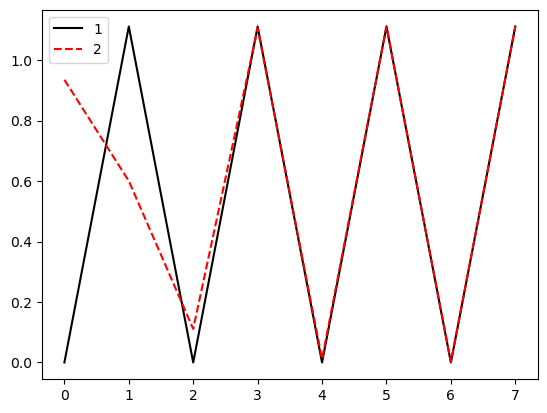
\includegraphics[width=0.5\linewidth]{posencoding.png}
  \caption{Positional encoding vectors for the position 1 (first) and 2 for 8-dimensional embedding vectors.}
  \label{fig:posencoding}
  \end{center}
\end{figure}


\begin{ack}
This work would not be possible without my tenure in Tampere
University. This position allows me to allocate time to projects
that interest myself and I want to share my findings to thank the
academic society and Finnish government. If you find this article or
related code useful, please cite this work (ArXiv link, author name,
and the title).

Universities all around the world are wonderful place for people like
me. I hope that the corporation thinking and style of management will
not destroy these institutes that were developed for more than one
thousand years.
\end{ack}

\printbibliography

\end{document}
